\newcommand{\FigSensMuMomentum}{%
\begin{figure}[bt]
\centering 
%\fbox{
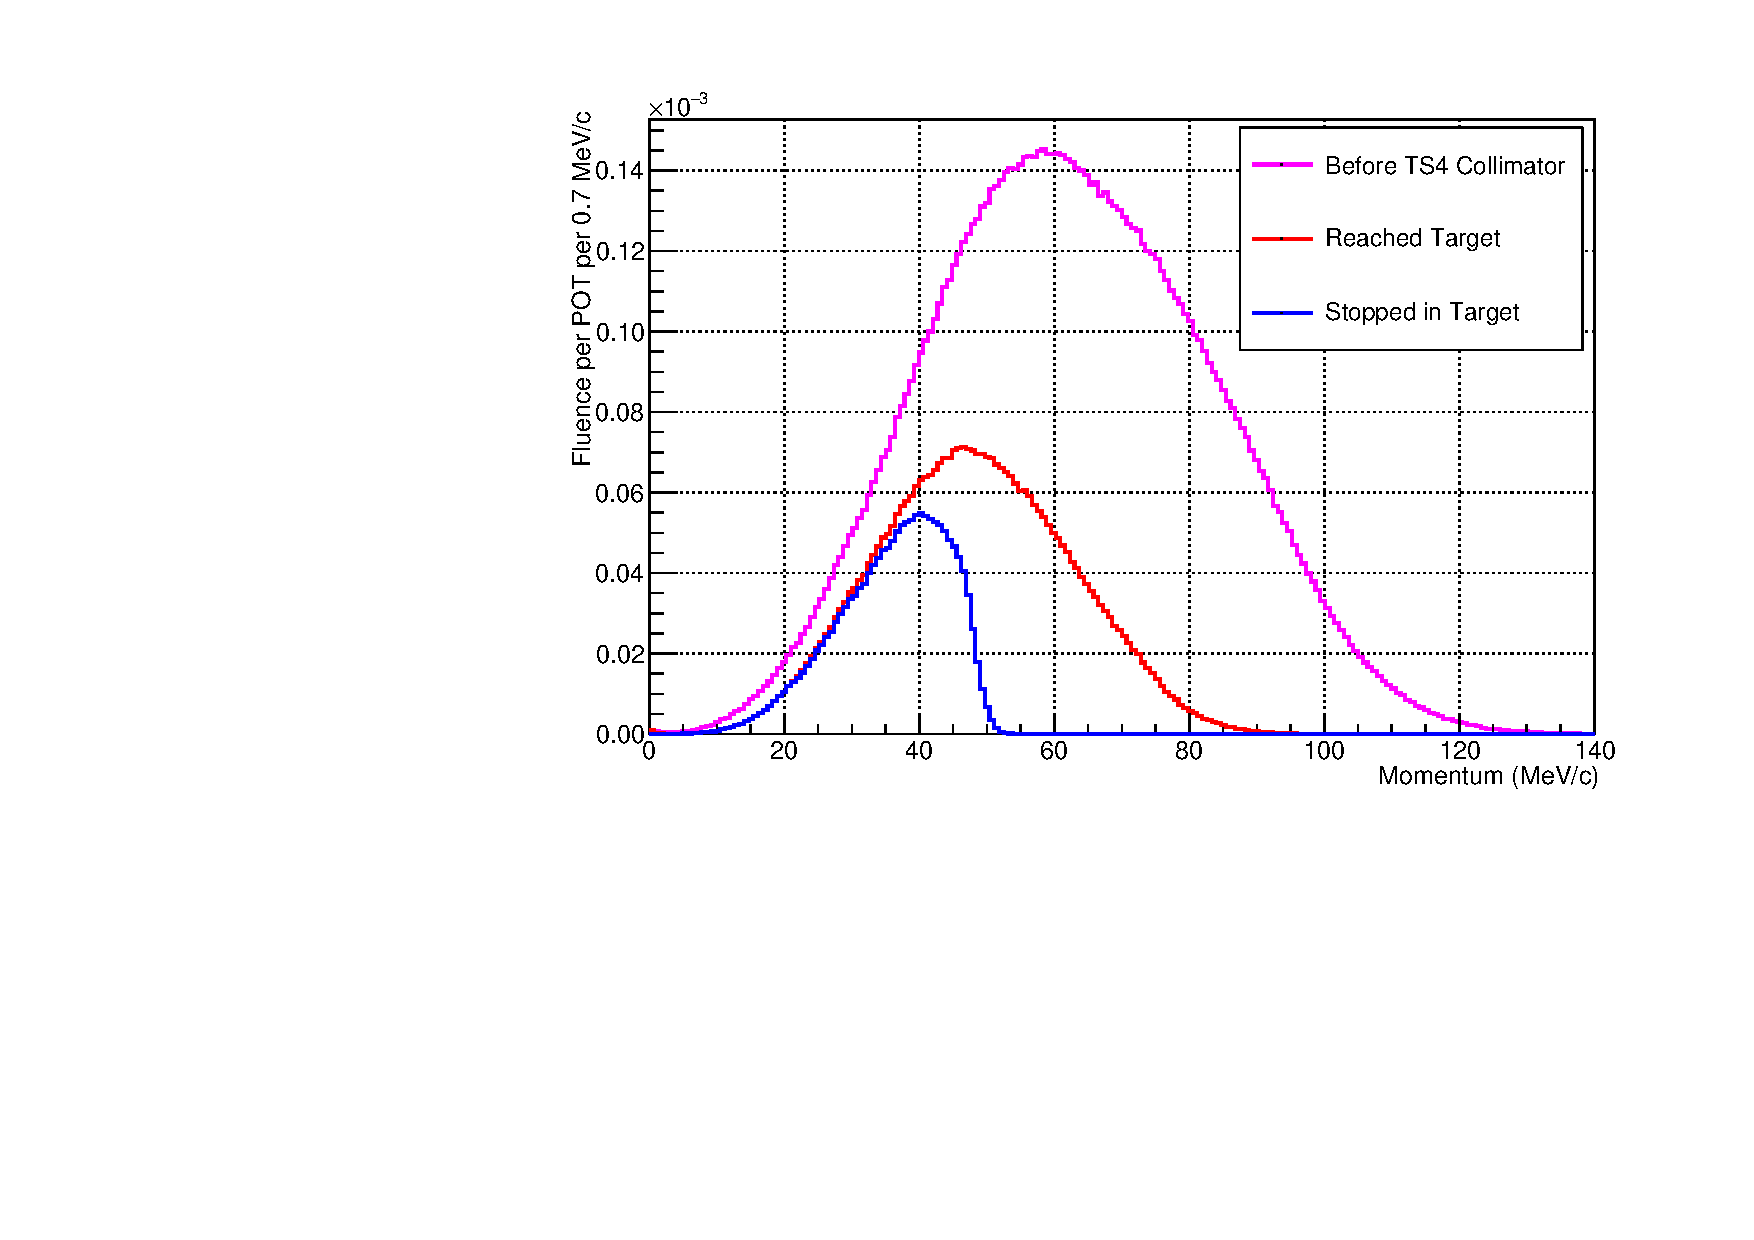
\includegraphics[width=0.8\textwidth,trim=0.5cm 0.1cm 1.5cm 0.8cm,clip]{figs/sensitivity/Muon_momentum.pdf}
%}
\caption{\figlabel{sense:muMomenta}
The Momentum and rates of muons reaching the final beam collimator, the stopping target, and actually stopping in the target.
It can be seen how the present target geometry is unable to stop muons of greater than around 50~MeV/c.
}
\end{figure}\xspace}

\newcommand{\FigSensMuStopsTwoD}{%
\begin{figure}[tb]
\centering 
\subfloat[\figlabel{sense:stops:XZ}X-Z plane]{
        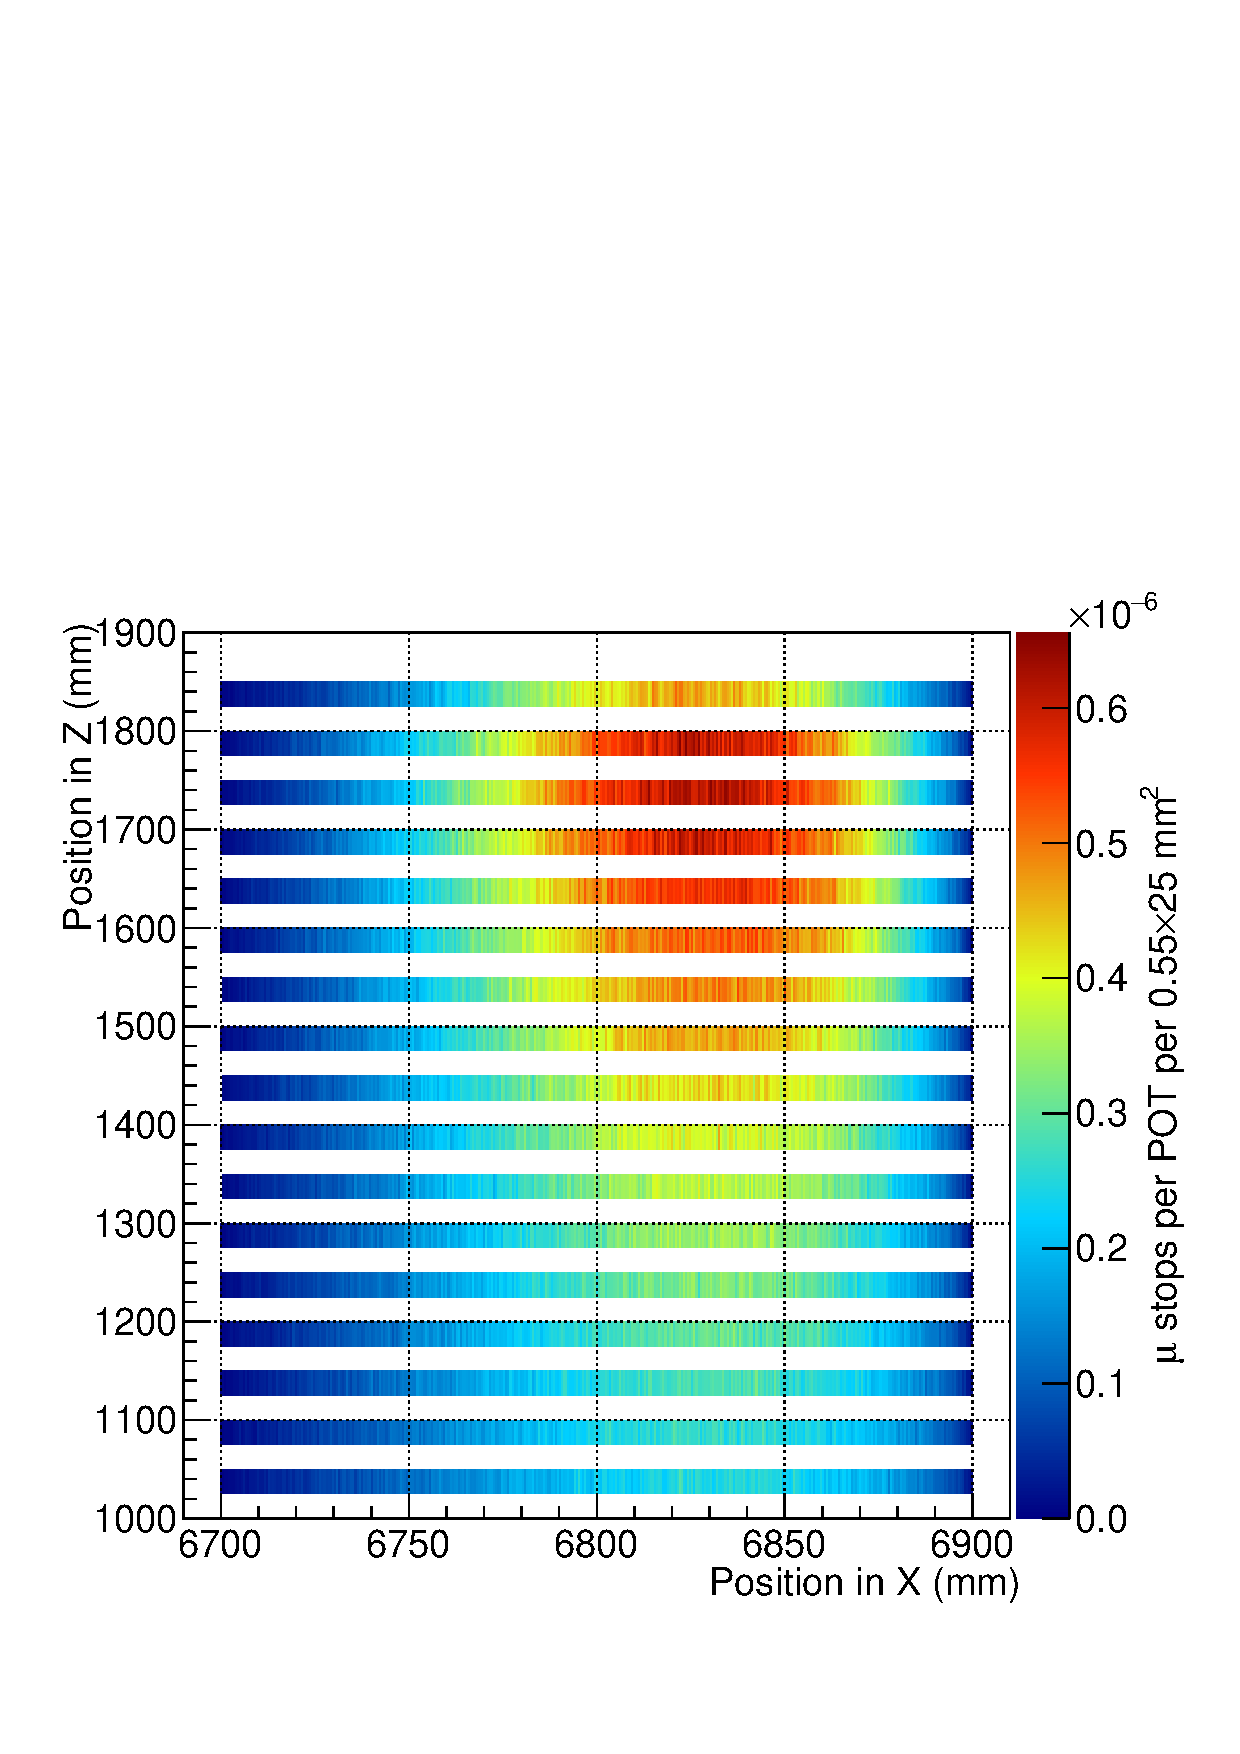
\includegraphics[width=0.33\textwidth,trim=0.3cm 1.5cm 0.7cm 1.2cm,clip]{figs/sensitivity/MuStops_2D_XZ.pdf}}
\subfloat[\figlabel{sense:stops:XY}X-Y plane]{
	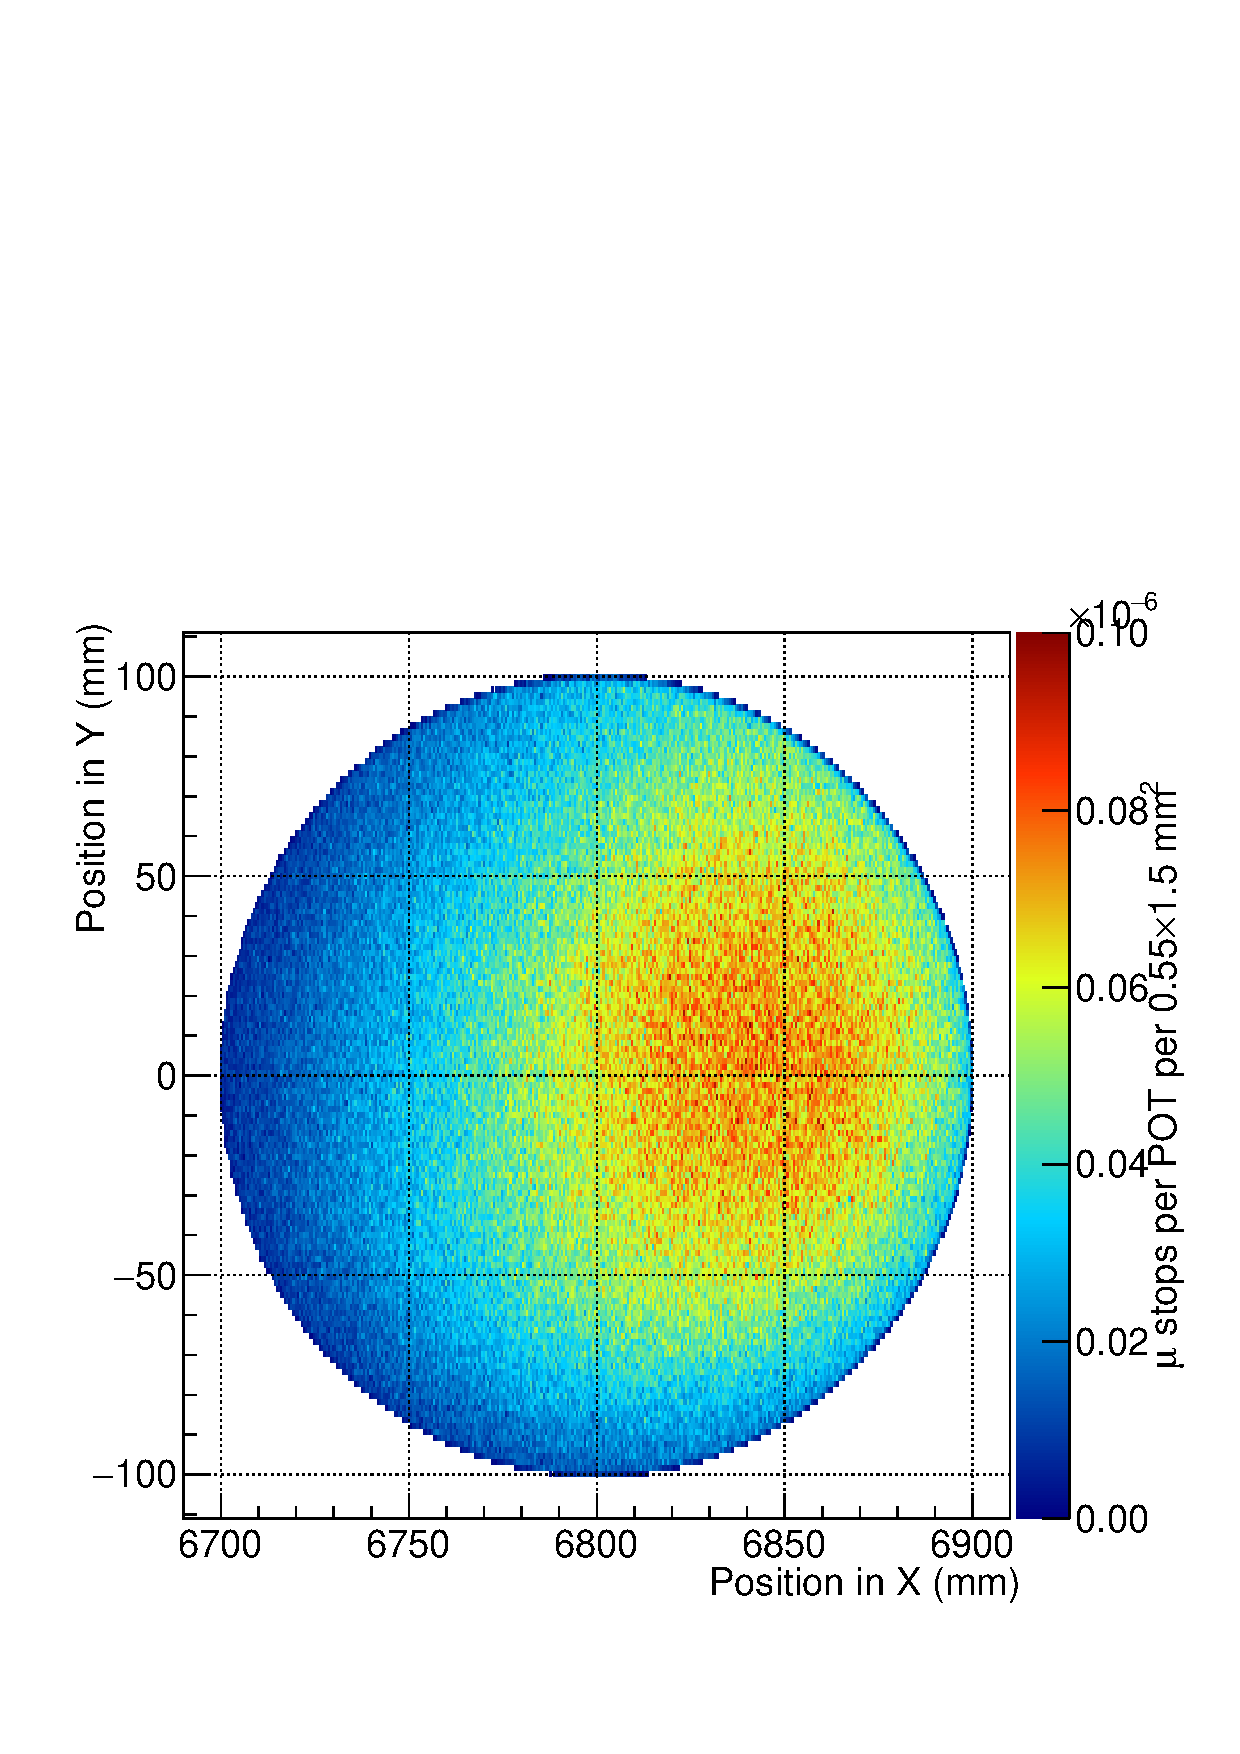
\includegraphics[width=0.33\textwidth,trim=0.3cm 1.5cm 0.7cm 1.2cm,clip]{figs/sensitivity/MuStops_2D_XY.pdf}}
\subfloat[\figlabel{sense:stops:ZY}Z-Y plane]{
	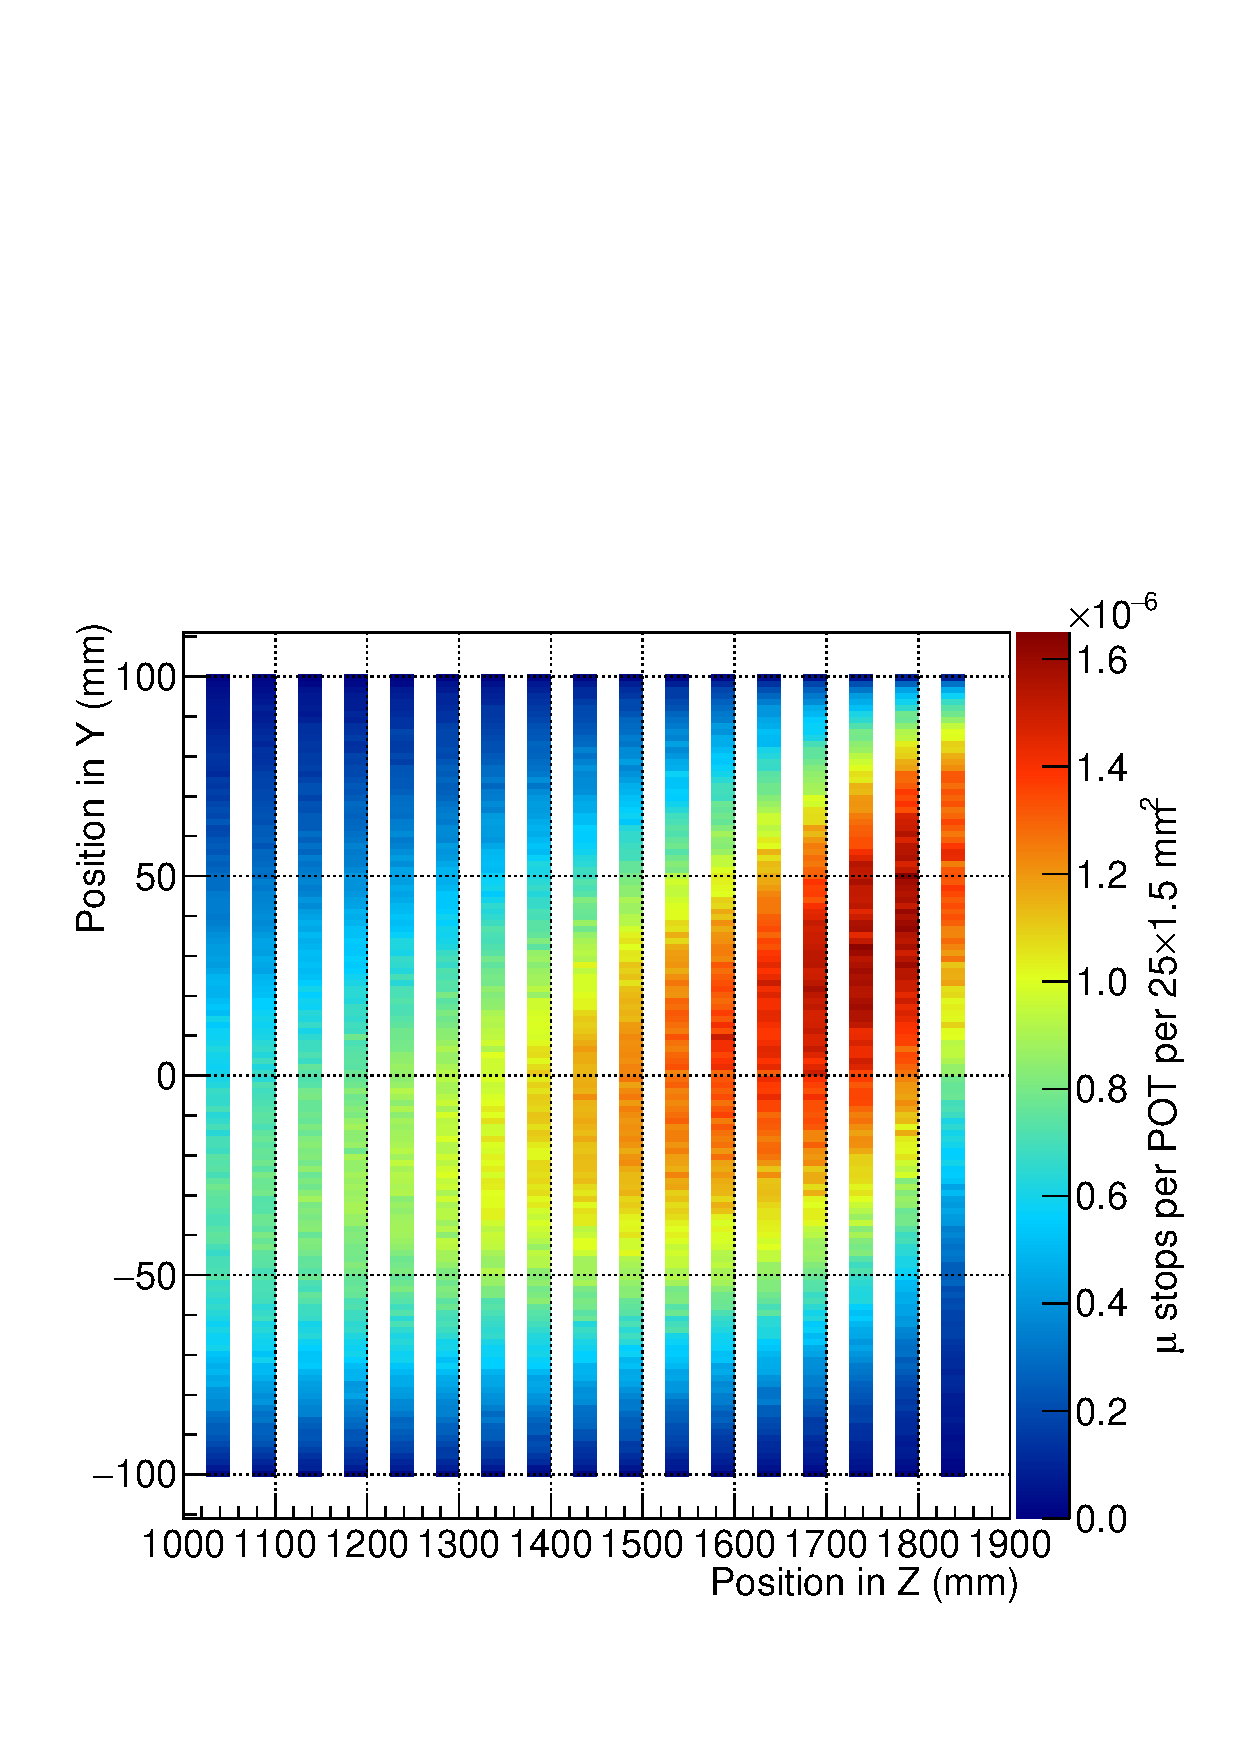
\includegraphics[width=0.33\textwidth,trim=0.3cm 1.5cm 0.7cm 1.2cm,clip]{figs/sensitivity/MuStops_2D_ZY.pdf}}
\\
\subfloat[\figlabel{sense:stops:X}X axis]{
	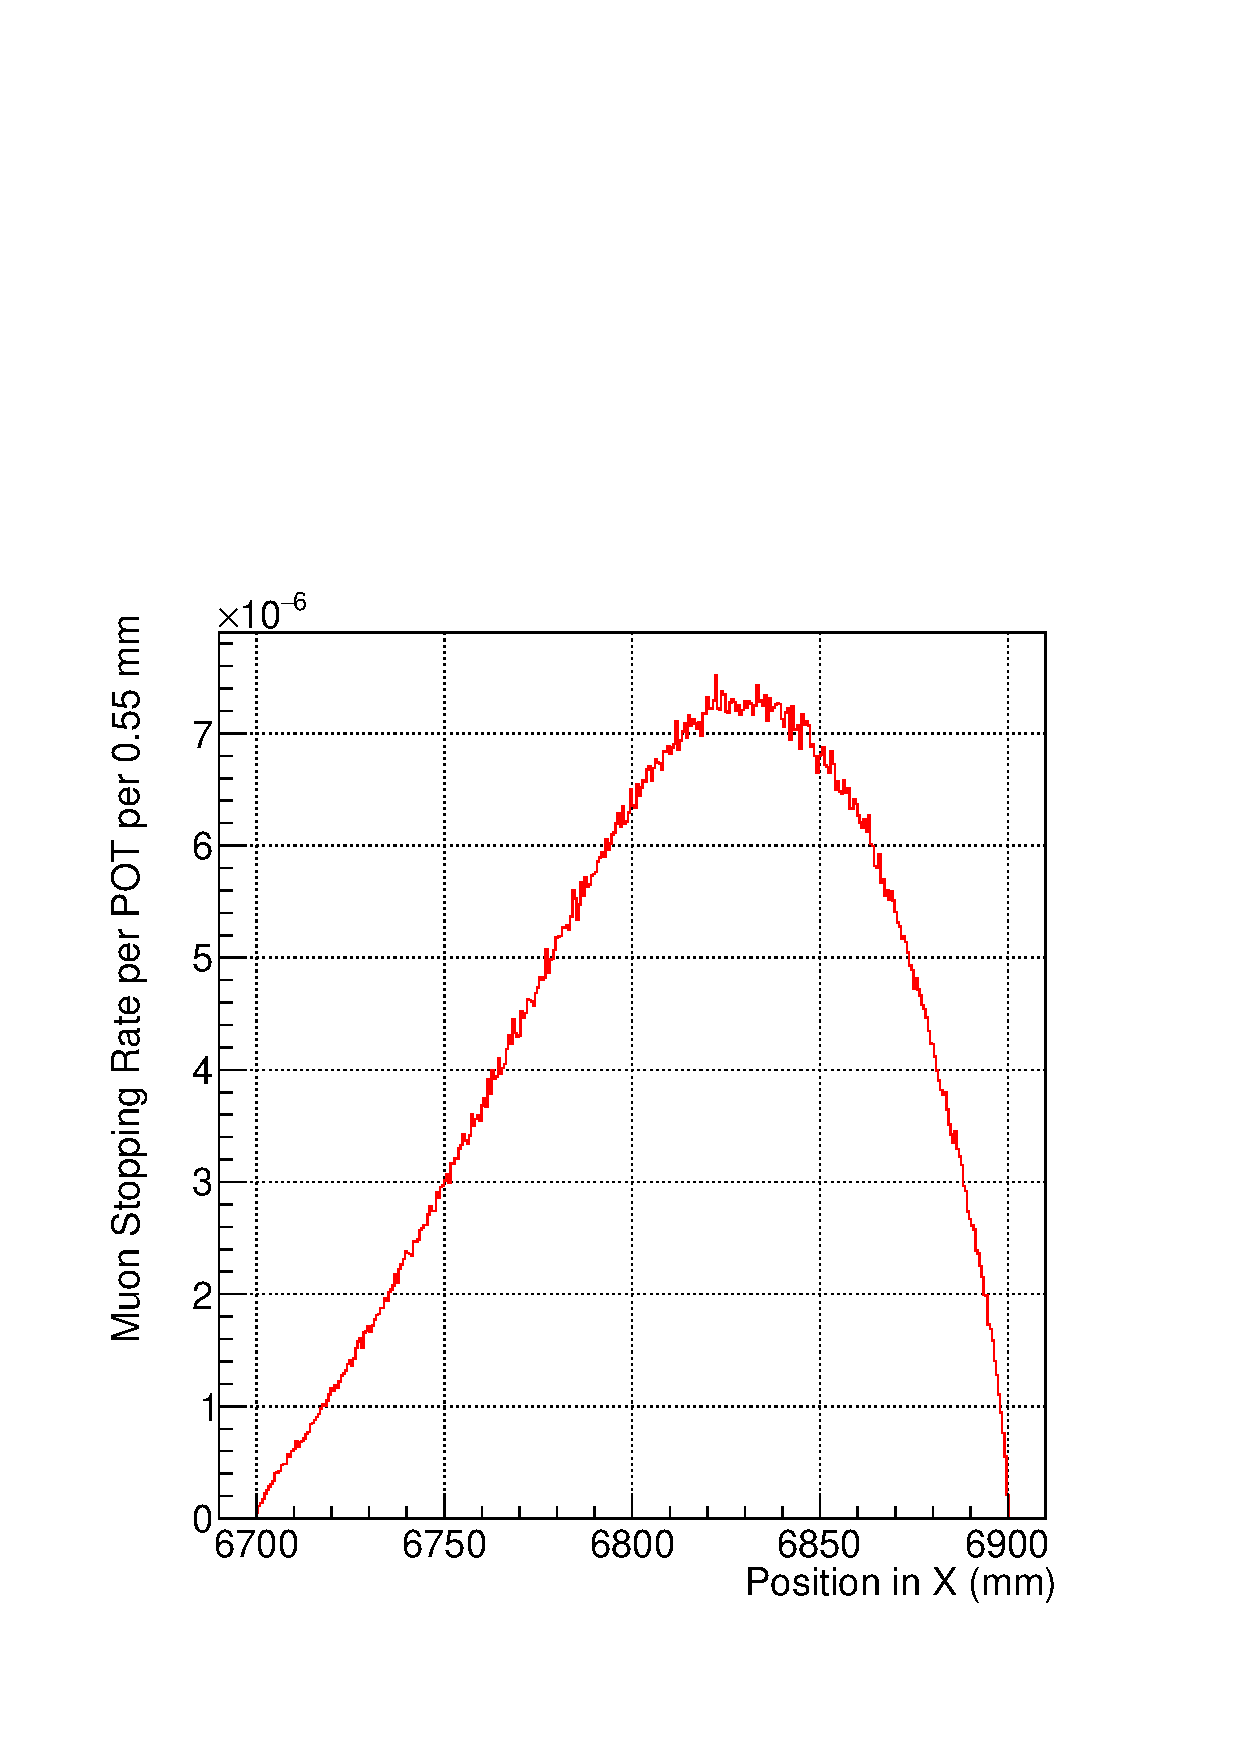
\includegraphics[width=0.33\textwidth,trim=0.3cm 1.5cm 0.7cm 1.2cm,clip]{figs/sensitivity/MuStops_1D_X.pdf}}
\subfloat[\figlabel{sense:stops:Y}Y axis]{
	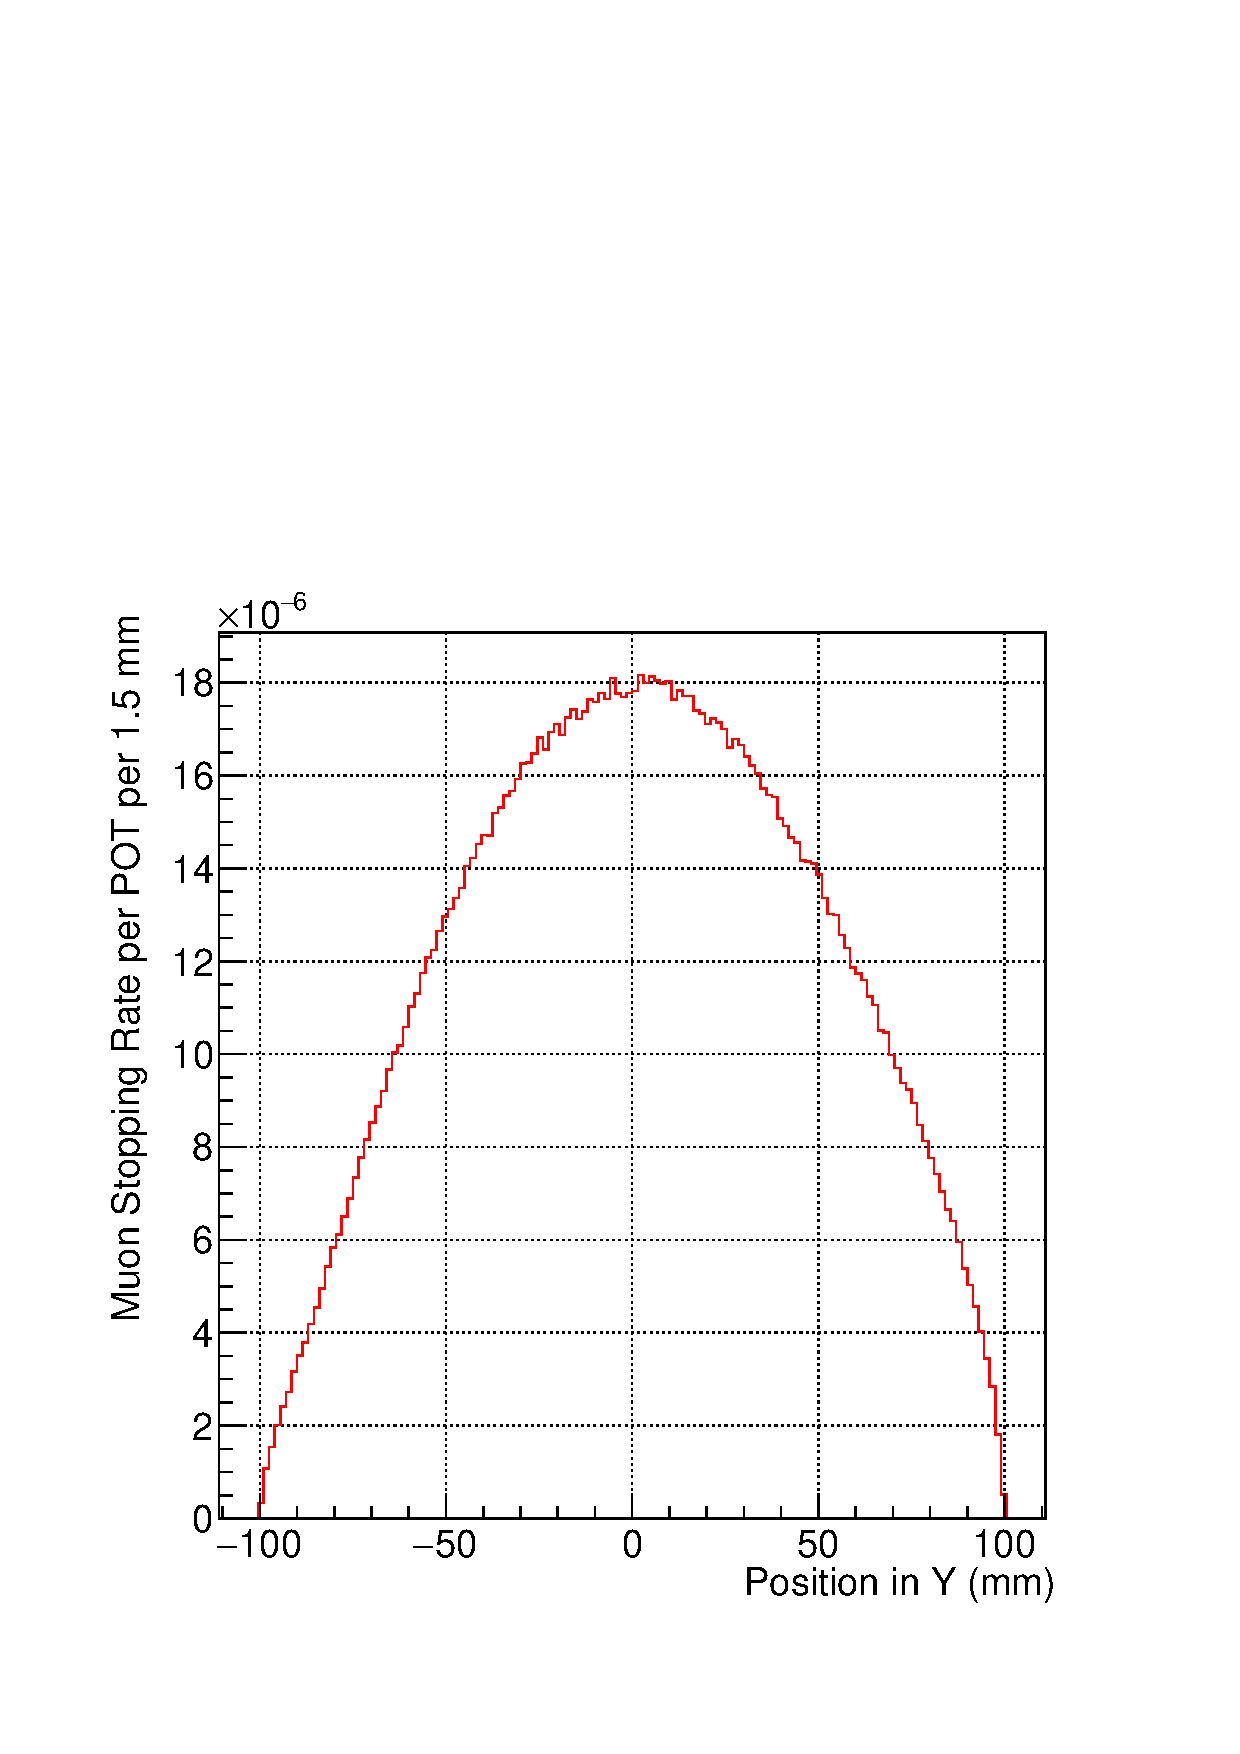
\includegraphics[width=0.33\textwidth,trim=0.3cm 1.5cm 0.7cm 1.2cm,clip]{figs/sensitivity/MuStops_1D_Y.pdf}}
\subfloat[\figlabel{sense:stops:Z}Z axis]{
        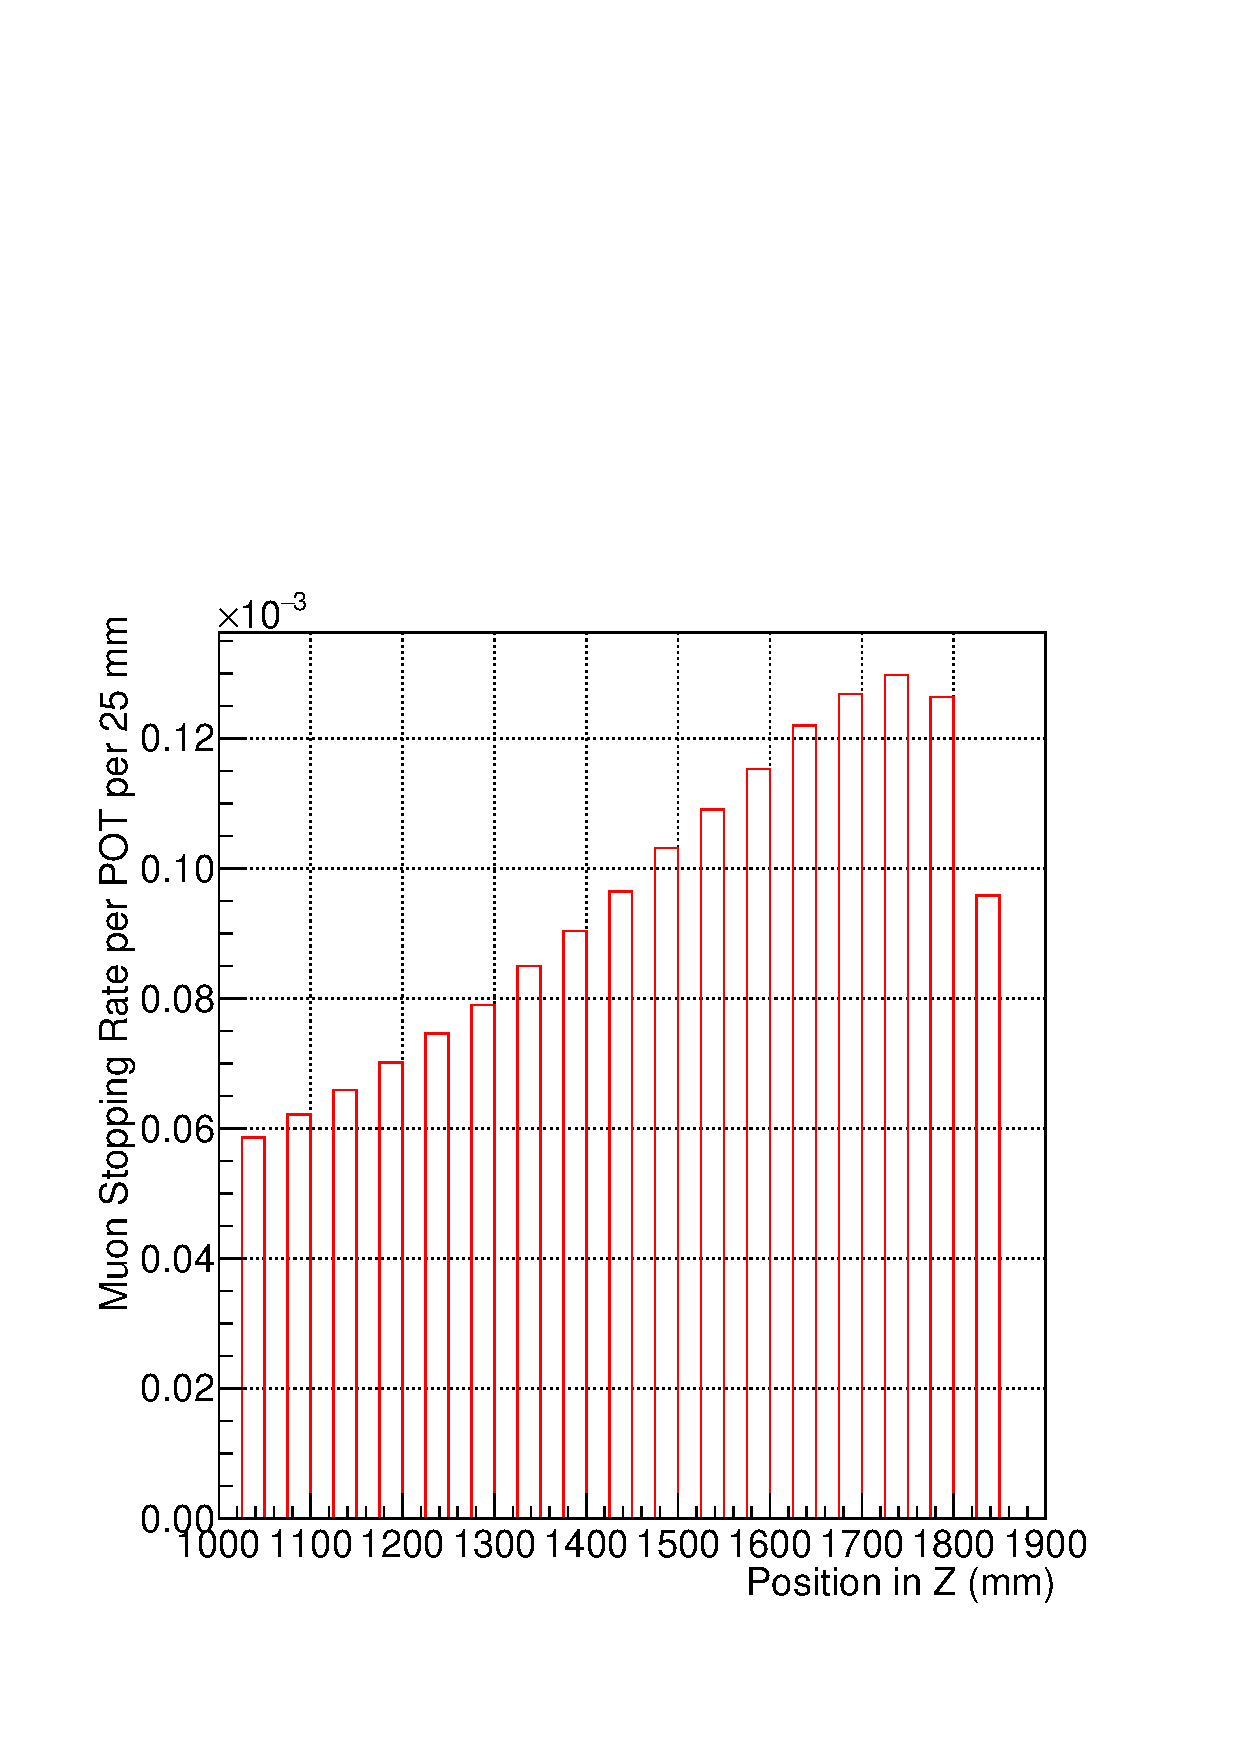
\includegraphics[width=0.33\textwidth,trim=0.3cm 1.5cm 0.7cm 1.2cm,clip]{figs/sensitivity/MuStops_1D_Z.pdf}}
\caption{\figlabel{sense:stops}
Projections of the final position of stopped muons in the stopping target.
	Axes are from the SimG4 global coordinate system, so that $+X$ points away from the production target, $+Y$ is vertically upwards, and $+Z$ is the direction of the muon beam at the production target.
	The muon beam in these plots is therefore travelling in the negative-$Z$ direction having passed around through 180\degree of the bent solenoid.
}
\end{figure}\xspace}

\newcommand{\FigSensGeomAccept}{%
\begin{figure}[bt]
\centering 
\subfloat[\figlabel{sense:accept:height}Path of Signal Electrons in the Beamline Projection]{
	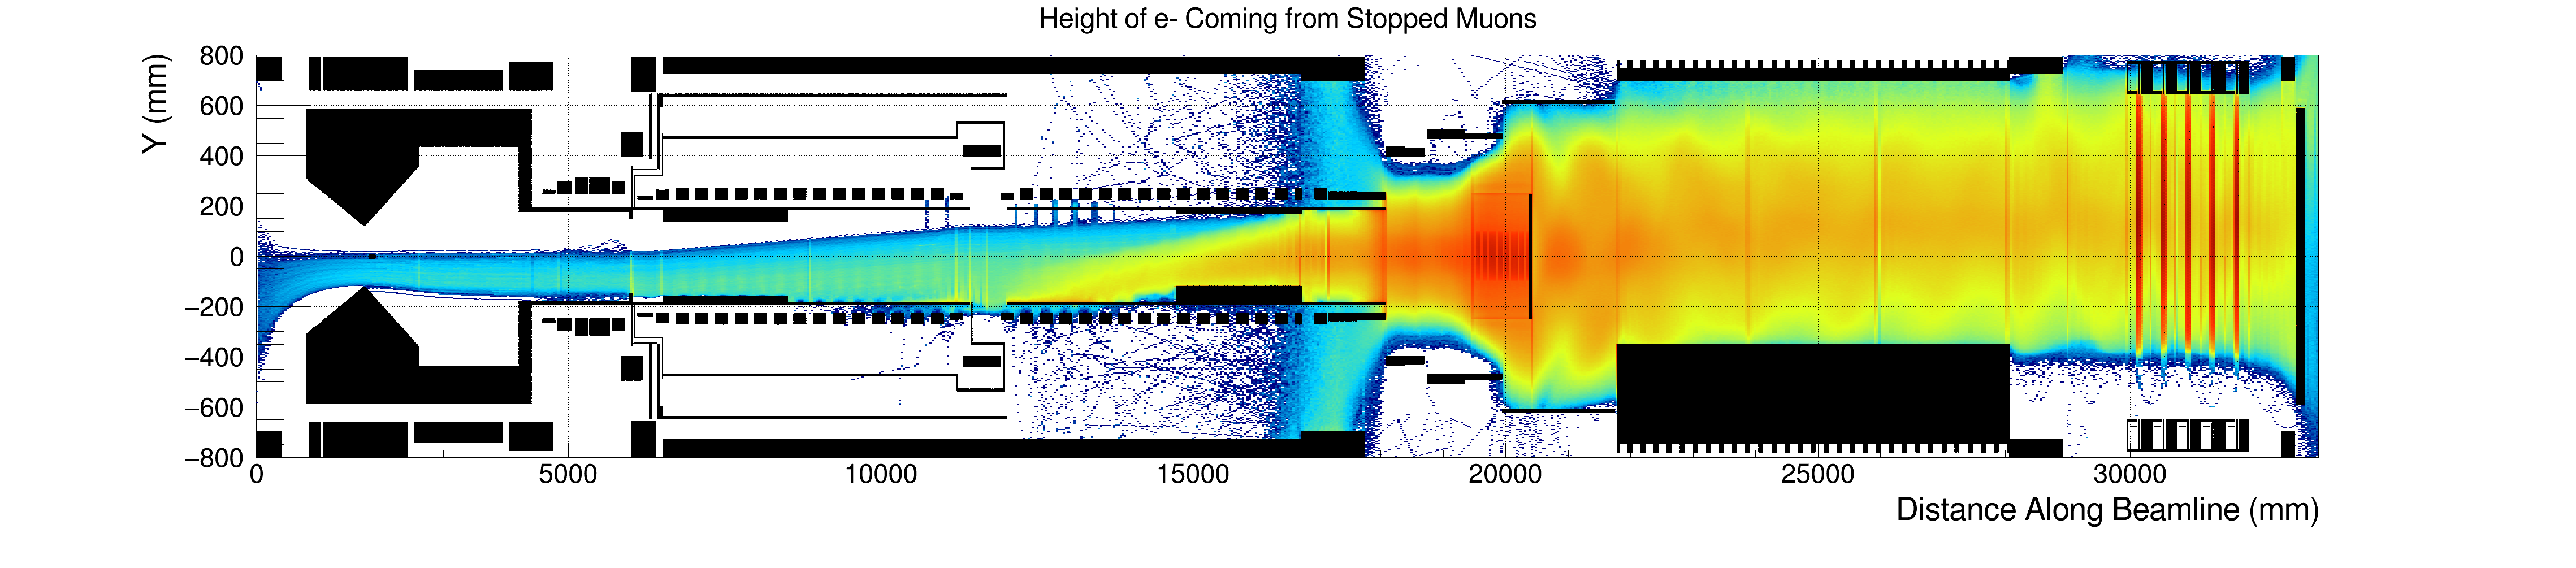
\includegraphics[width=0.99\textwidth,trim=8.3cm 1.5cm 13.2cm 2.2cm,clip]{figs/sensitivity/Tidied_SignalHeight2DVsBeamline.png}}\\
\subfloat[\figlabel{sense:accept:flux}Survival Probability for Signal Electrons]{
        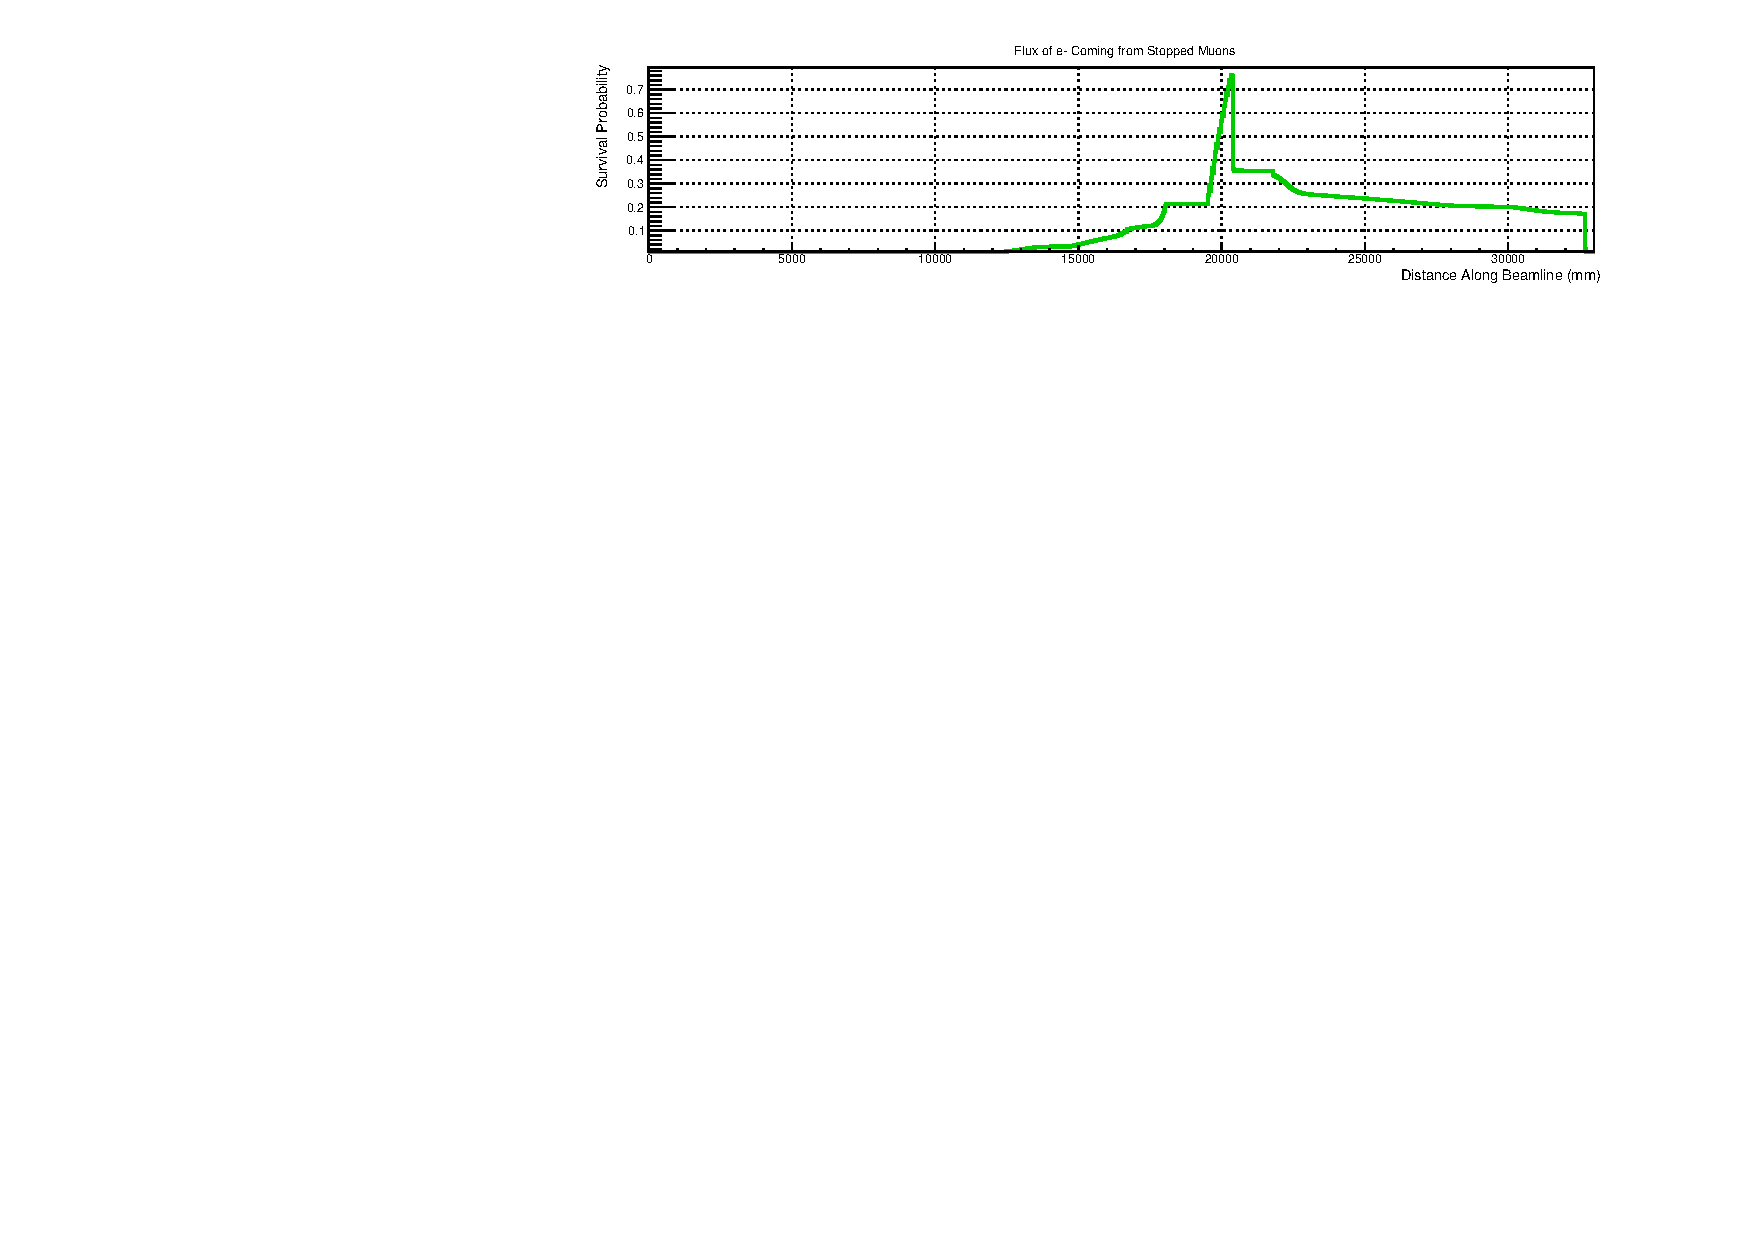
\includegraphics[width=0.99\textwidth,trim=1.0cm 0.2cm 1.7cm 0.4cm,clip]{figs/sensitivity/Tidied_SignalSurivivalVsBeamline.pdf}}
\caption{\figlabel{sense:accept}
Geometric acceptance of signal events.
\protect\subref{fig:sense:accept:height} Projection of the trajectories of signal electrons to the surface formed by the beamline axis and the vertical direction.
\protect\subref{fig:sense:accept:flux} Survival probability of signal electrons as a function of the distance along the beamline axis.
The x-axis range is the same in the two plots.
From these, it is clear how the acceptance is diminished by the DIO blocker in the spectrometer, although from that point on the rate of signal loss reduces.
}
\end{figure}\xspace}

\newcommand{\FigSensMomTransfer}{%
\begin{figure}[tb]
\centering 
%\fbox{
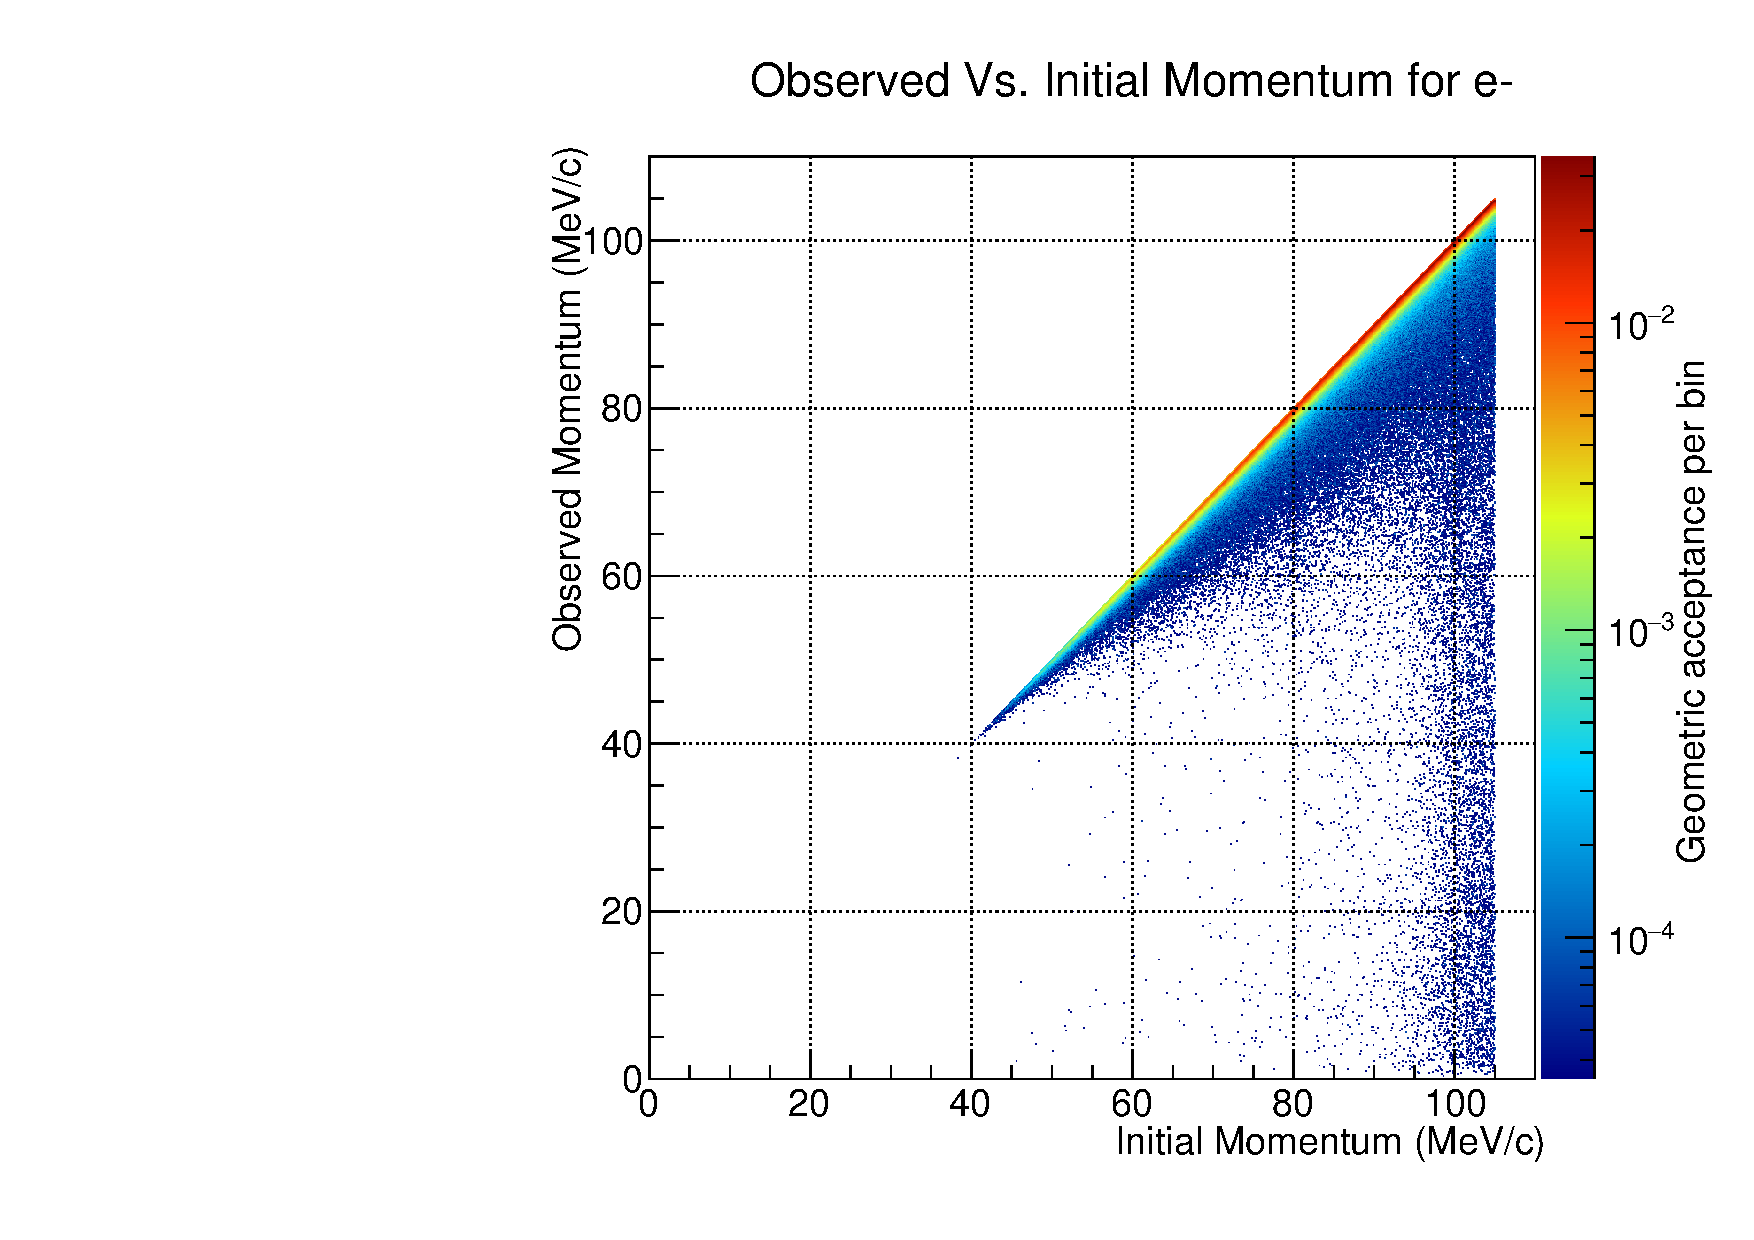
\includegraphics[width=0.5\textwidth,trim=0.0cm 0.0cm 0.0cm 1.6cm,clip]{figs/sensitivity/MomentumTransfer.pdf}
%}
\caption{\figlabel{sense:momTransfer}
The transfer matrix for electrons originating at the target, including the geometric acceptance and energy loss.
}
\end{figure}\xspace}

\newcommand{\FigSensMomSpectra}{%
\begin{figure}[tb]
\centering 
%\fbox{
\subfloat[Incl.~energy loss\figlabel{sense:spectra:ELoss}]             {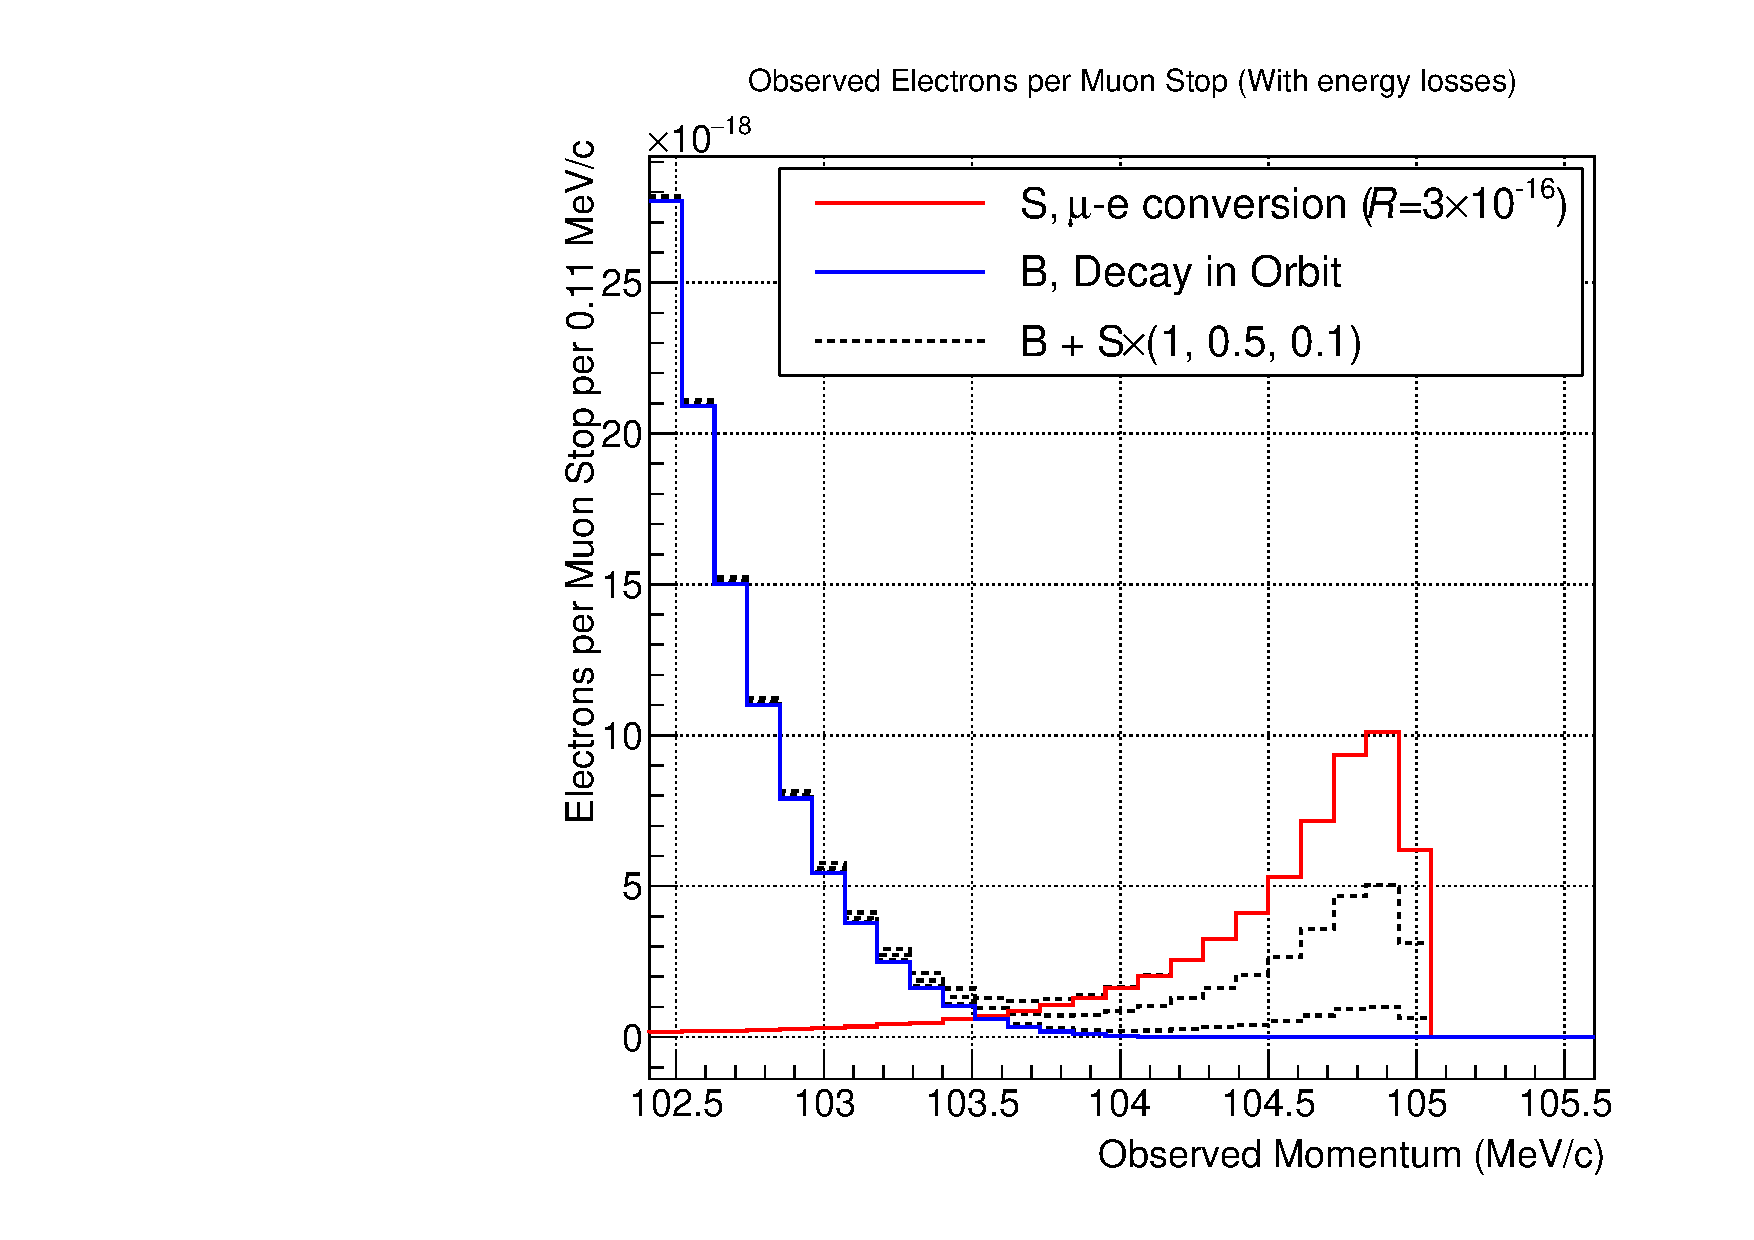
\includegraphics[width=0.48\textwidth,trim=0.0cm 0.0cm 1.0cm 1.0cm,clip]{figs/sensitivity/ConversionVsDio_Spectra.pdf}}
\subfloat[Energy loss \& resolution\figlabel{sense:spectra:resolution}]{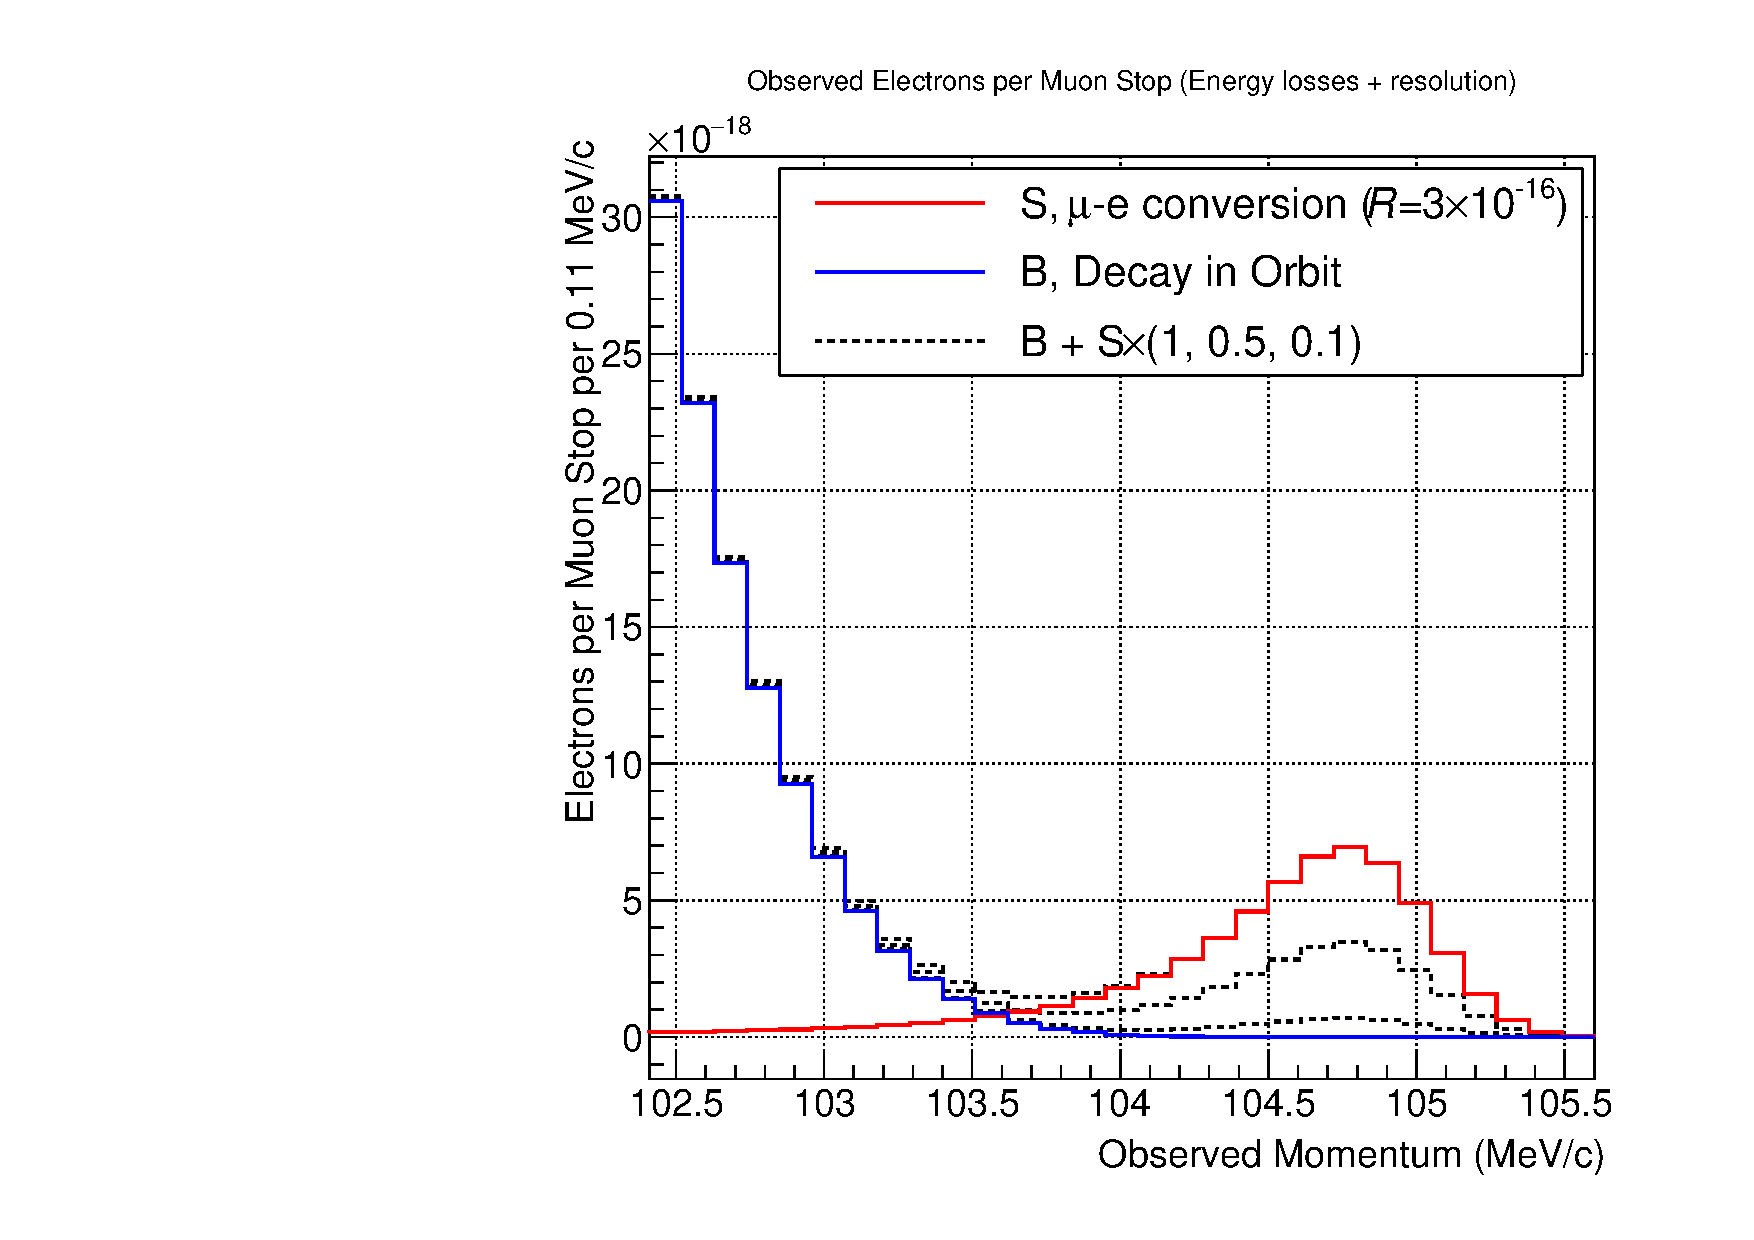
\includegraphics[width=0.48\textwidth,trim=0.0cm 0.0cm 1.0cm 1.0cm,clip]{figs/sensitivity/ConversionVsDio_Spectra-wResolution.pdf}}
\caption{
The spectrum of electrons coming from \ac{DIO} and \mueconv assuming a conversion rate of $\mathcal{R}=\sci{3}{-16}$.
Black dashed lines indicate the total electron distribution that would be seen (the sum of $S$ and $B$) if the signal has the assumed conversion rate of \num{3e-16}, half that rate, and one tenth that rate.
\protect\subref{fig:sense:spectra:ELoss} Includes energy losses in the target, beamline, and detector;
\protect\subref{fig:sense:spectra:resolution} also includes resolution effects (for a Gaussian resolution function with a standard deviation of $\sigma=200$~keV/c).
\figlabel{sense:spectra}}
\end{figure}\xspace}

\newcommand{\FigSensMomIntegral}{%
\begin{figure}[tb]
\centering 
%\fbox{
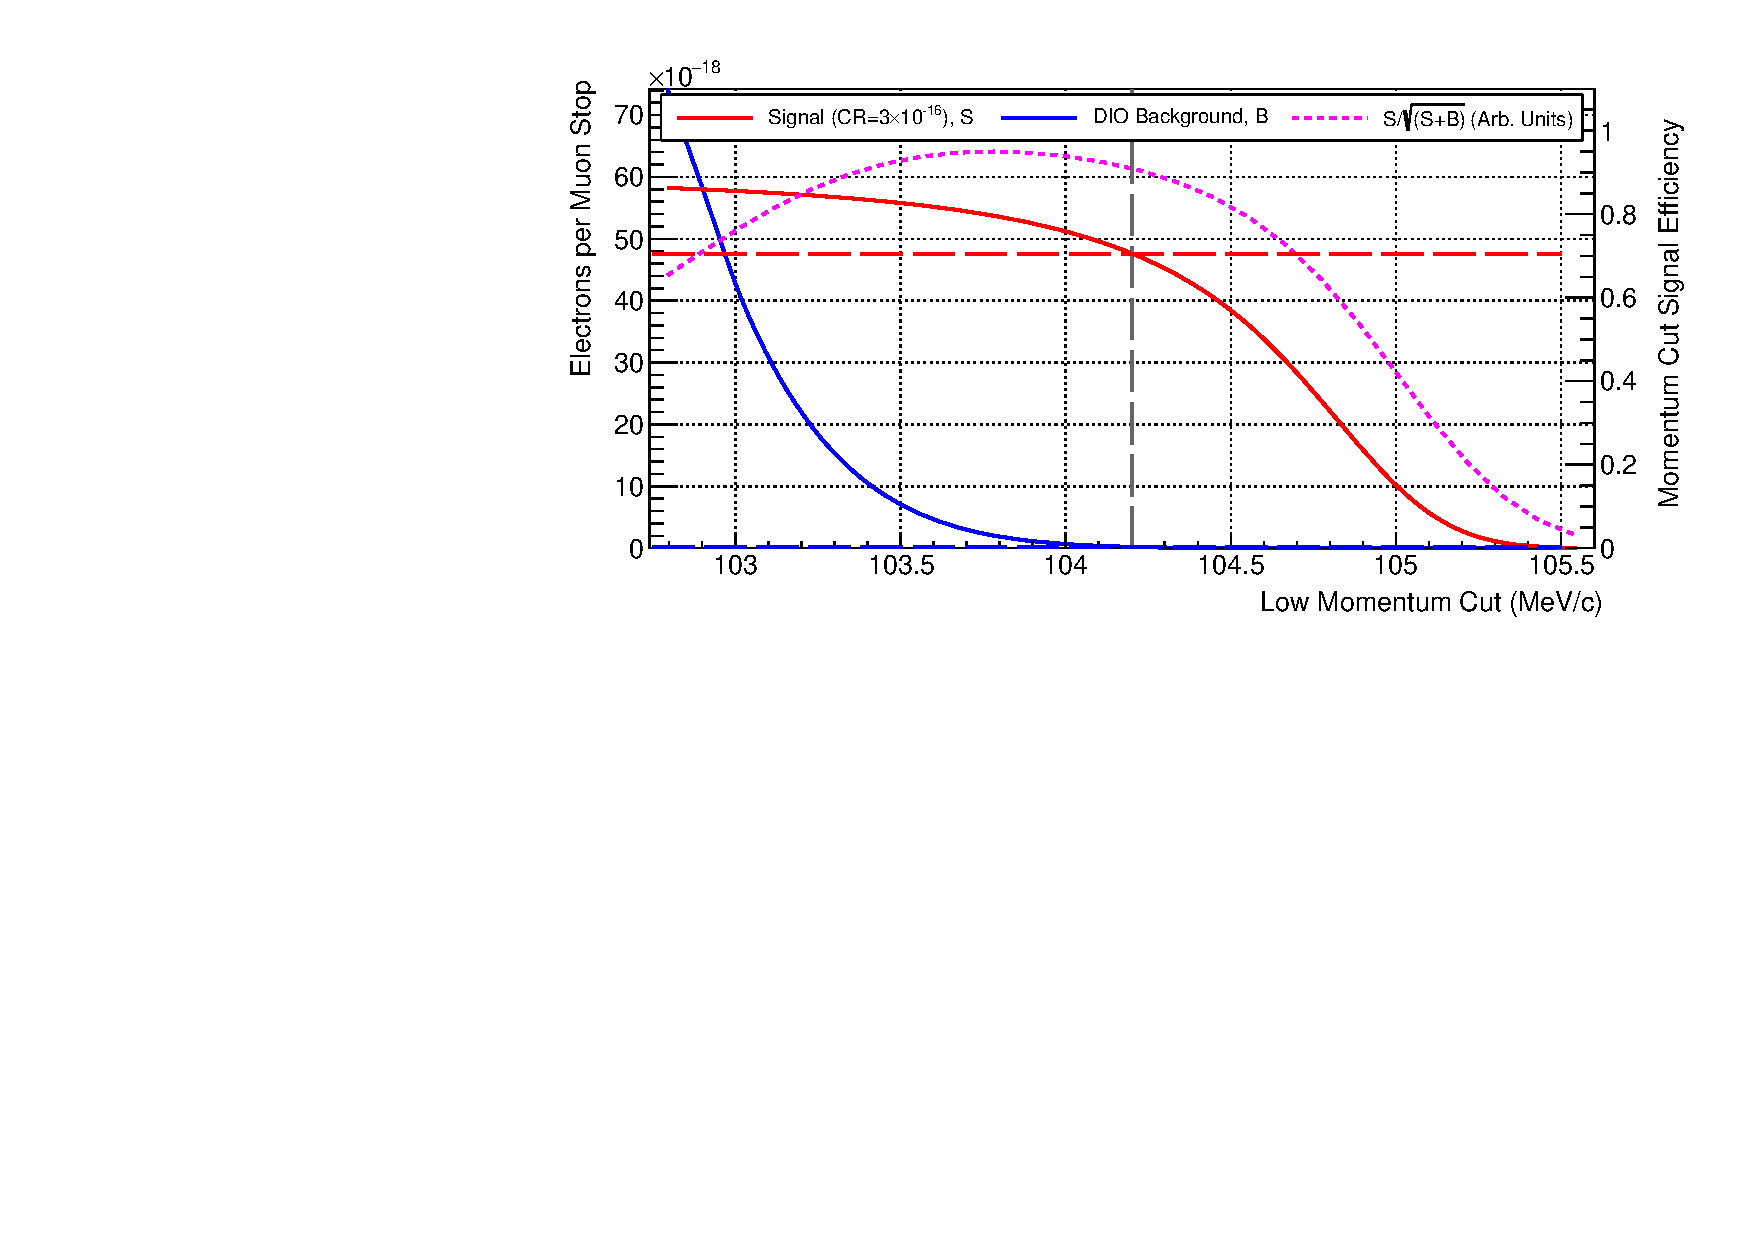
\includegraphics[width=0.99\textwidth,trim=0.5cm 0.0cm 0.5cm 0.3cm,clip]{figs/sensitivity/ConversionVsDio_Integrated.pdf}
%}
\caption{\figlabel{sense:integral}
Relative signal versus \ac{DIO} background as a function of the low-momentum cut value assuming a conversion rate of $\mathcal{R}=\sci{3}{-16}$.
The magenta line is the signal over square root of signal plus background for this conversion rate shown as an indicator of the optimum cut value.
}
\end{figure}\xspace}

\newcommand{\FigSensTiming}{%
\begin{figure}[b]
\centering 
%\fbox{
\subfloat[\figlabel{sense:timing:signal}Signal Arrival Time]      {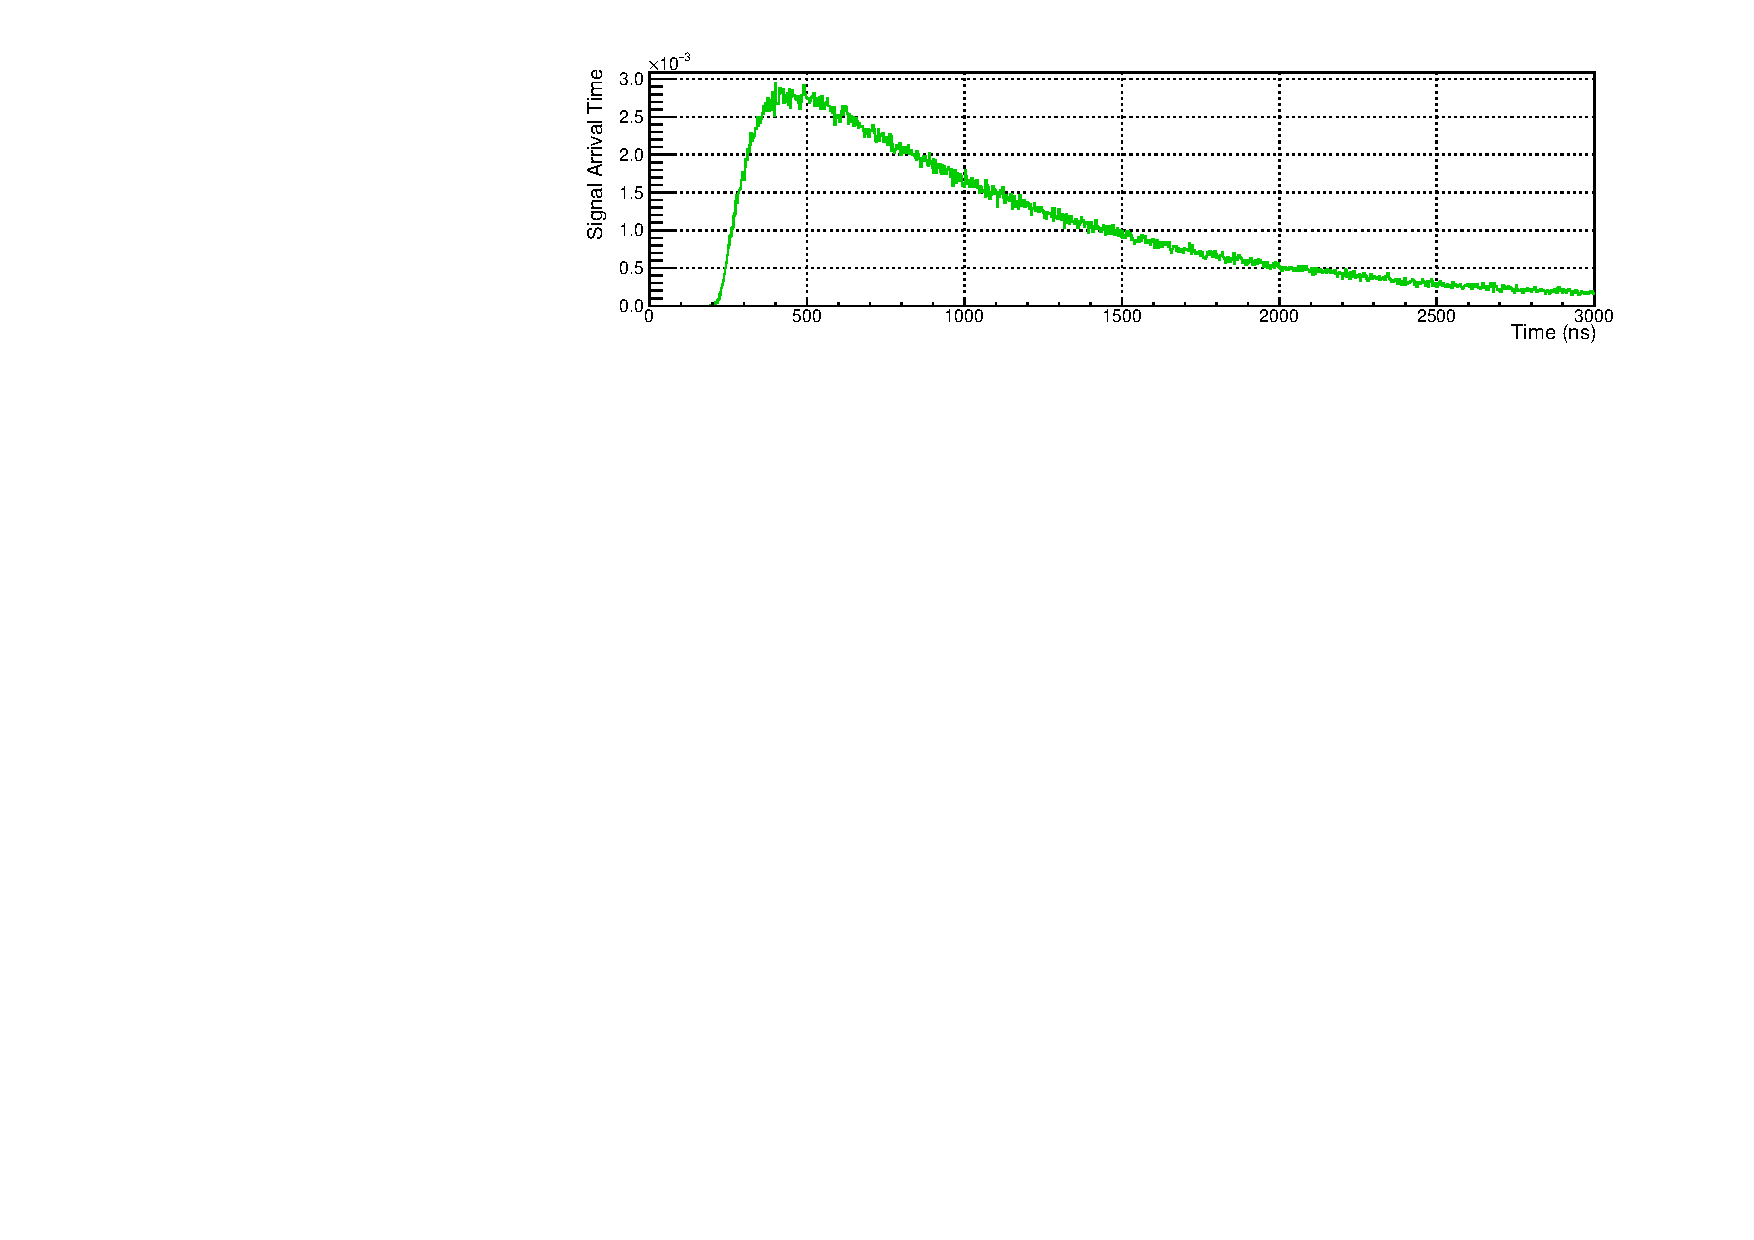
\includegraphics[width=0.9\textwidth,trim=0.9cm 0.1cm 1.5cm 0.20cm,clip]{figs/sensitivity/160823_MuonLifetime.pdf}}\\
\subfloat[\figlabel{sense:timing:efficiency}Timing Cut Efficiency]{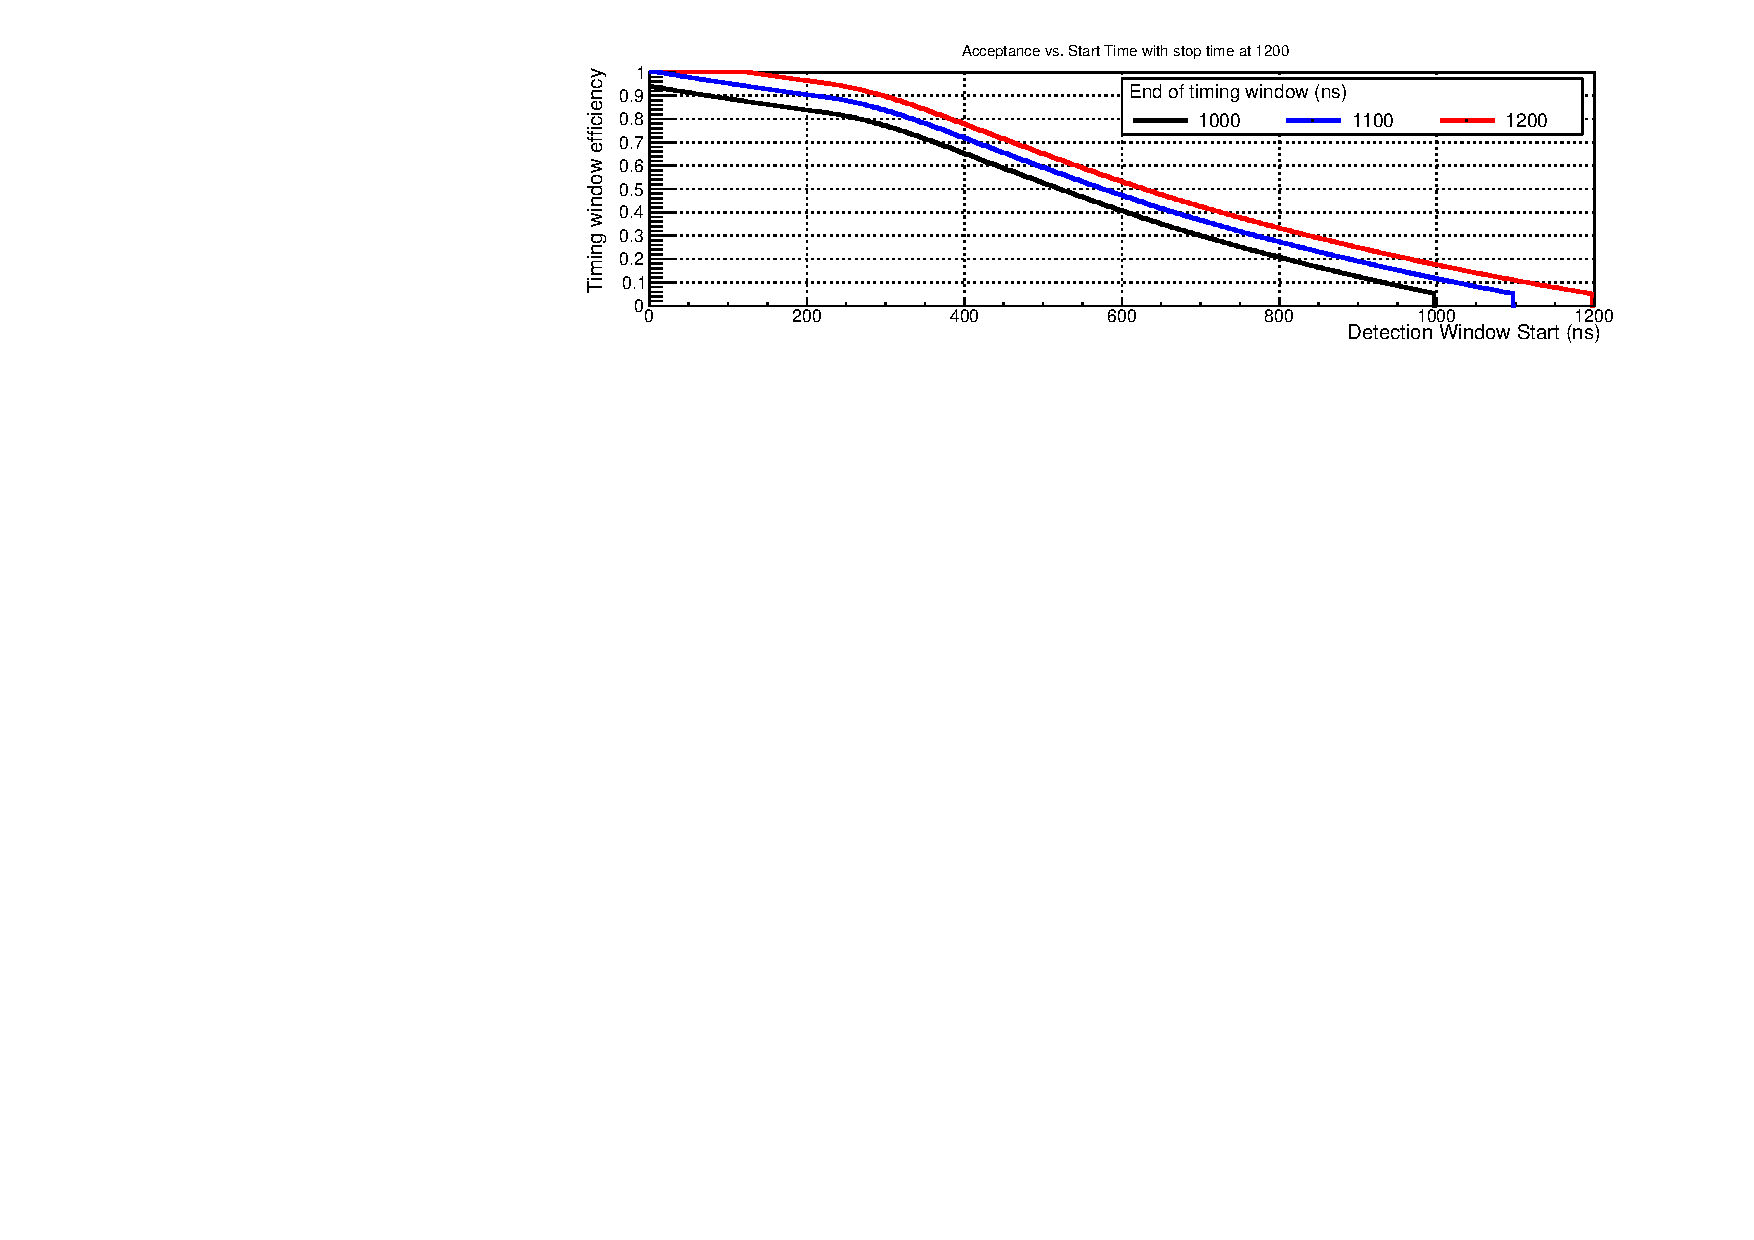
\includegraphics[width=0.9\textwidth,trim=0.9cm 0.1cm 1.5cm 0.4cm,clip]{figs/sensitivity/160823_TimingCutEfficiency.pdf}}
\caption{\figlabel{sense:timing}
Timing of signal electrons.
\protect\subref{fig:sense:timing:signal} The arrival time of signal electrons at the detector, including the effect of the proton pulse width, particle transportation, and the muon lifetime.
\protect\subref{fig:sense:timing:efficiency} the efficiency of the timing window as a function of the switch-on time.  Assumes a pulse separation of 1.17~$\mu$s.
}
\end{figure}\xspace}

\newcommand{\TabSensParams}{%
\begin{table}[b]
\centering
\begin{tabular}{lll}
	\hline
         $I_p$                          & 7~$\mu$A & Proton beam current                            \\ 
	 ${R}_{\mu/p}$      & \VarMuStopsPerPOT & Muon stopping rate per POT                     \\ 
%	 $f_\mathrm{1s}$                & 90\%    & Probability of reaching the ground state \\ 
	 $\mathcal{B}_\mathrm{capture}$ & 61\%    & Branching ratio for muon nuclear capture in Al \\ 
	 $A_{\mu\rightarrow e}$         & \VarTotalSignalAcceptance   & Total signal acceptance of \phaseII            \\ 
	\hline
\end{tabular}
        \caption{\tablabel{sense:ses}
        Parameters that determine the run time and single event sensitivity for COMET \phaseII based on this study.
        }
\end{table}\xspace}

\newcommand{\TabSensEstimates}{%
\begin{table}[t]
\centering
	\begin{tabular}{L{0.25\textwidth}p{0.14\textwidth}S[table-format=2.1]p{0.12\textwidth}p{0.23\textwidth}}
	\hline
							& Single event sensitivity & \multicolumn{1}{p{0.13\textwidth}}{Total \acp{POT} ($\times10^{19}$)} &Beam time $t_\textrm{run}$ (s) & SES in one year of continuous beam \\ 
  \hline
  COMET \phaseII\hspace{1ex}(this study)                & \VarPredictedSES         & 68.3 & \VarRunTime[3]                  & \VarPredictedSESPerYear                         \\ 
  COMET \phaseII\hspace{1ex}(CDR 2009~\cite{CDRphase2}) & \sci{2.6}{-17}           & 85   & \sci{2.00}{7}                  & \sci{1.65}{-17}                         \\ 
  Mu2e~\cite{Mu2e2014}                                  & \sci{2.4}{-17}           & 36   & \sci{6.00}{7}                  & \sci{4.57}{-17}                         \\ 
  COMET \phaseI~\cite{TDR2016}                          & \sci{3.0}{-15}           & 3.2 & \sci{1.26}{7}                  & \sci{1.19}{-15}                         \\ 
	\hline
\end{tabular}
        \caption{\tablabel{sense:comparisons}
        Comparison between the run time and single-event sensitivity from this study and from the 2009 CDR, the \phaseI TDR, and  the Mu2e experiment's TDR.
	The \ac{ses} in one year of continuous beam is the single-event-sensitivity that can be achieved in \num{3.15e7}~seconds of running, assuming no beam shutdown periods.
        }
\end{table}\xspace}
